\documentclass{article}

\usepackage[margin=0.75in, headheight=35pt, includehead, includefoot]{geometry}

\usepackage{fancyhdr}
\usepackage[T1]{fontenc}
\usepackage[shortlabels]{enumitem}
\usepackage{graphicx}
\graphicspath{ {./} }
\usepackage[export]{adjustbox}
\usepackage{booktabs}
\usepackage{forest}
\usepackage{listings}
\lstset{escapeinside={(*@}{@*)}}

\setlength{\parindent}{4em}
\setlength{\parskip}{1em}

\pagestyle{fancy}
\rhead{Alex Kitsul\\230134210\\February 2, 2021}

\begin{document}
\thispagestyle{empty}
\begin{center}
\topskip0pt
\vspace*{\fill}
\Huge Alex Kitsul\\
\Huge 230134210\\
\Huge CPSC 450\\
\Huge Assignment 2 - Report\\
\Huge February 2\\
\vspace*{\fill}
\end{center}
\pagebreak

\section*{Psedocode}
\begin{lstlisting}
main:
	k <- from file
	d <- from file
	pairs <- from file
	
	pairs <- debruijin_pairs(pairs)
	graph <- glue_pairs(pairs)
	
	while flat_answer is invalid:
		answer <- eulerian_cycle(graph[i])
		dimensional_answer <- interpret_answer(answer, d)
		flat_answer = flatten_answer(dimensional_answer)
		reset_answer(graph)
		i += 1
		
	display flatanswer
	
reset_visited(graph):
	for all nodes in graph:
		for all edges in node:
			visited = false
			
make_pairs(pairs):
	list of debrujin_pairs

	for every pair in pairs:
		prefix 1 <- all but the last letter of pair[0]
		suffix 1 <- all but the first letter of pair[0]
		
		prefix 2 <- all but the last letter of pair[1]
		suffix 2 <- all but the first letter of pair[1]
		
		prefix <- prefix 1, prefix 2
		suffix <- suffix 1, suffix 2
		
		node <- prefix, suffix, pair
		
		add node to debrujin pairs
		
glue_pairs(debruijin_pairs):
	compare all node prefixes with other node suffixs in debruijin_pairs for matches
		if there's a match, add an edge
		
	find a start and end node if applicable
	
	compare all node prefixes to see if there are matches
		if there are matches:
			take all pointers from del_node and append to current
			take all pointers from del_node - 1 and point to current
			
eulerian_cycle(start_vertex):
	*** MODIFIED FROM SLIDES ***
	form a Cycle by randomly walking from start (avoiding already visited edges)
	while Cycle is not Eulerian
		select a node newStart in Cycle with still unexplored outgoing edges   
		form a Cycle_p by traversing Cycle from newStart and randomly walking afterwards  
		Cycle <- Cycle_p 
return Cycle

interpret_answer(answer, d):
	2D_Array <- []

	for all pairs in answer:
		find pair from edge
		chararray <- chararray + offset by number of chararrays (rows)
		chararray <- chararray + pair[0]
		chararray <- chararray + offset by d
		chararray <- chararray + pair[1]
		chararray <- chararray + offset by spaces until at end column
		2D_Array append chararray
		
flatten_answer(2D_Array):
	flat_answer
	for all columns in 2D_Array:
		if every character in columns is the same:
			flat_answer <- flat_answer + character
		else:
			Answer is misaligned, did not start on the right node
			return to eularian_cycle
		
\end{lstlisting}

\pagebreak

\section*{Program Code}
\textbf{\underline{Read-Pairs-Reconstruction.py}}
\begin{lstlisting}
from Node import Node

def main():
    file_input = input("Enter file name: ")

    # File preparation stuff, gets data from file and then parses it to usable variables
    with open(file_input, "r") as file:
        file_digits = file.readline()
        file_digits_split = file_digits.split(" ")

        file_pairs = file.read()
        file_pairs_splitline = file_pairs.split("\n")
        file_pairs_splitpairs = []

        for pair in file_pairs_splitline:
            file_pairs_splitpairs.append(pair.split("|"))
       
        try:
            k = int(file_digits_split[0])
            d = int(file_digits_split[1])
        except:
            print("Unable to parse k and d, please check these values and try again")
            exit()

        # Main Driver for application
        debruijin_pairs = make_pairs(file_pairs_splitpairs)
        graph = glue_pairs(debruijin_pairs)

        i = 0
        flat_answer = -1

        # If our answer is misaligned, we did not use the correct start node, retry from a different node
        while(flat_answer == -1):
            answer = eulerian_cycle(graph[i])
            dimensional_answer = interpret_answer(answer, d)
            flat_answer = flatten_answer(dimensional_answer)
            reset_visited(graph)
            i += 1

        print(flat_answer)

def reset_visited(graph):
    """
        Resets all the visit flags for nodes supplied in graph 

        Parameters:

            graph (list[Node]): a list of Nodes

        Returns:

            None: Modifies objects directly
    """
    for i in graph:
            map = i.getVisitedMap()
            for j in map:
                map[j] = 0

def make_pairs(pairs):
    """
        Parses the data into the usable pairs of k-1 length

        Parameters:

            pairs (list[list]): a list of k-mer pairs
                Example: [["GAGA", "TTGA"], ["TCGT", "GATG"]]

        Returns:

            debruijn_pairs (list[Node])
    """
    debruijn_pairs = []
    for pair in pairs:
        # Make first prefix and suffix using pair[0]
        prefix_1 = pair[0][:-1]
        suffix_1 = pair[0][1:]

        # Make second prefix and suffix using pair[1]
        prefix_2 = pair[1][:-1]
        suffix_2 = pair[1][1:]

        # Append the prefix's and suffix's to their lists and make them into a Node object,
        # and append to list of Nodes
        prefix = [prefix_1, prefix_2]
        suffix = [suffix_1, suffix_2]
        node = Node(prefix, suffix, pair)
        debruijn_pairs.append(node)

    return debruijn_pairs

def glue_pairs(pairs):
    """
        Takes a list of debruijn pairs and ties them together using Node getNext and getPrev methods
        After tieing them together, checks for similar nodes, and ties them together

        Parameters:

            pairs (list[Node]): A list of debrujin pair nodes to be tied together

        Returns:

            start_node (Node): The first Node in the path
    """
    # Ties nodes together in one contig strand
    for node in pairs:
        for other_node in pairs:
            if (other_node != node):
                if (node.getSuffix() == other_node.getPrefix() and not node.getNext() and not other_node.getPrev()):
                    # Then are a match!
                    node.addNext(other_node)
                    other_node.addPrev(node)
                    node.addPair(other_node, node.getPair())
                    node.addVisited(other_node)
                    # Found match, don't need to continue
                    break

    # If there's a start and end node, needs to be made into a cycle by pointing the end at the beginning
    start_node = None
    end_node = None

    for node in pairs:
        if (not node.getPrev()):
            start_node = node
        if (not node.getNext()):
            end_node = node

    if (start_node and end_node):
        end_node.addNext(start_node)
        end_node.addPair(start_node, end_node.getPair())
        end_node.addVisited(start_node)

    # Iterate through the node list, take the current node and check all occurances after it in the list for matching prefixes
    end = len(pairs)
    for i in range(len(pairs)):
        j = i + 1
        while (j < end):
            # If we have a match
            if(pairs[i].getPrefix() == pairs[j].getPrefix()):
                # Take all the pointers from the Node to be deleted, and append them to the current node
                pairs[i].appendNext(pairs[j].getNext())
                pairs[i].addPairMap(pairs[j].getPairMap())
                pairs[i].addVisitedMap(pairs[j].getVisitedMap())

                # Take the pointers that point to the matching Node, and point them to the new current Node
                pairs[j].getPrev()[0].changeNext(pairs[j], pairs[i])
                pairs[j].getPrev()[0].changeVisited(pairs[j], pairs[i])
                pairs[j].getPrev()[0].changePairMap(pairs[j], pairs[i])
                # Remove the matching node from the list
                pairs.pop(j)
                end -= 1
            j += 1

    return pairs

def eulerian_cycle(start_vertex):
    """
        Calculates Eulerian cycle of Nodes from the start_node

        Parameters:
            start_node (Node): The beginning Node in the De Bruijn Graph, can be random in this case

        Returns:
            answer: (list[Node]): The ordered list of Nodes to be interpreted (could be incorrect if start node was wrong)
    """
    cycle = []
    cycle_prime = []
    node_with_extra_edges = [start_vertex]

    # While cycle is not Eulerian
    while (node_with_extra_edges):
        current_vertex = node_with_extra_edges[0]
        node_with_extra_edges.remove(current_vertex)
        flag = 1
        # Form a cycle by randomly walking in balanced graph
        while(flag):
            not_visited = []
            for i in current_vertex.getNext():
                if (not current_vertex.isVisited(i)):
                    not_visited.append(i)
            if (not_visited):
                current_vertex.setVisited(not_visited[0])
                cycle_prime.append(current_vertex)
                current_vertex = not_visited[0]
            else:
                flag = 0

        # Stuck, loop to find nodes with unused edges, if none, then we are Eularian
        for i in cycle_prime:
            map = i.getVisitedMap()
            for j in map:
                if (map[j] == 0):
                    node_with_extra_edges.append(j)
                    break

        cycle = cycle_prime

    return cycle

def interpret_answer(answer, d):
    """
        Interprets the ordered list of Nodes and parses it to a 2D matrix

        Parameters:

            answer (list[Node]): The list of Nodes in order to interpret
            d (int): Distance between read-pairs

        Returns:

            dimensional (list[list[char]]): a 2D representation of the read pairs
    """
    dimensional = []
    offset = 0
    extra_spaces = len(answer) - 1

    for i in (range(len(answer))):
        # Get current Node's pairmap
        map = answer[i].getPairMap()
        # Get the next Node's prefix
        
        pair = None
        # If the map is populated (not the last object in the de Bruijn graph)
        try:
            next_pref = answer[i + 1]
            # Search the map for the edge's pair
            for next in map:
                if (next == next_pref):
                    pair = map.get(next)
                    break
        except:
            # Else we're on the last node, get the last edge
            pair = answer[i].getPair()

        # Build a dimension of the array
        chararray = []
        # Pad beginning with spaces length of offset
        for i in range(offset):
            chararray.append(" ")

        # Turn top pair into list of chars
        chararray.extend(list(pair[0]))

        # Pad distance between read pairs with spaces
        for i in range(d):
            chararray.append(" ")

        # Turn bottom pair into list of chars
        chararray.extend(list(pair[1]))

        # Pad with spaces the length of the longest pair
        for i in range(extra_spaces - offset):
            chararray.append(" ")

        offset += 1

        # Append it to the 2D array
        dimensional.append(chararray)

    return dimensional

def flatten_answer(dimensional):
    """
        Take the 2D array, and check every column to make sure it is the same character, if they are, return the flattened array

        Parameters:

            dimensional (list[list[char]]): 2D representation of the read-pairs

        Returns:

            answer (string): A string representing our re-assembed composition
    
    """
    answer = ""
    for i in range(len(dimensional[0])):
        current_char = None
        for j in range(len(dimensional)):
            if (current_char == None):
                if (dimensional[j][i] != " "):
                    current_char = dimensional[j][i]
            else:
                if (dimensional[j][i] != " " and dimensional[j][i] != current_char):
                    return -1

        answer += current_char

    return answer

if __name__ == "__main__":
    main()

\end{lstlisting}
\textbf{\underline{Node.py}}
\begin{lstlisting}
class Node:
    def __init__(self, prefix, suffix, pair):
        self.prefix = prefix
        self.suffix = suffix
        self.next = []
        self.prev = []
        self.pairMap = dict()
        self.visited = dict()
        self.pair = pair

    def __str__(self):
        return str(self.prefix) + " " + str(self.suffix)

    def addNext(self, node):
        self.next.append(node)

    def appendNext(self, list):
        self.next.extend(list)

    def removeNext(self, node):
        self.next.remove(node)

    def wipeNext(self):
        self.next = []

    def addPrev(self, node):
        self.prev.append(node)

    def getNext(self):
        return self.next
    
    def getPrev(self):
        return self.prev

    def getPrefix(self):
        return self.prefix

    def getSuffix(self):
        return self.suffix

    def addPair(self, node, pair):
        self.pairMap[node] = pair

    def addPairMap(self, map):
        self.pairMap.update(map)
    
    def getPairMap(self):
        return self.pairMap

    def getPairFromMap(self, node):
        return self.pairMap[node]

    def getPair(self):
        return self.pair

    def wipePairMap(self):
        self.pairMap = dict()

    def getVisitedMap(self):
        return self.visited
    
    def addVisited(self, node):
        self.visited[node] = 0

    def addVisitedMap(self, map):
        self.visited.update(map)
        
    def setVisited(self, node):
        self.visited[node] = 1

    def isVisited(self, node):
        return self.visited[node]

    def wipeVisited(self):
        self.visited = dict()

    def changeNext(self, old, new):
        for i in range(len(self.next)):
            if (self.next[i] == old):
                self.next[i] = new
            else:
                print("errr")

    def changeVisited(self, old, new):
        self.visited.pop(old)
        self.visited[new] = 0

    def changePairMap(self, old, new):
        key = self.pairMap.pop(old)
        self.pairMap[new] = key
    
\end{lstlisting}

\pagebreak

\section*{Examples with Output}
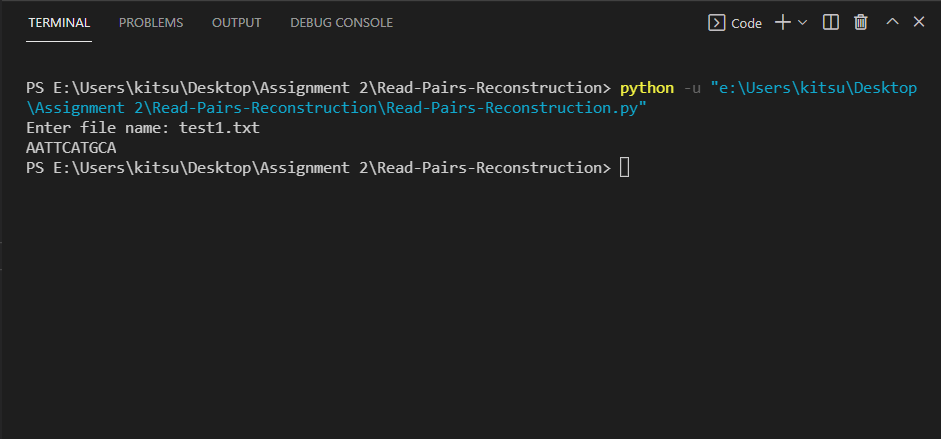
\includegraphics[scale=0.5]{ExampleInput1.png}\\
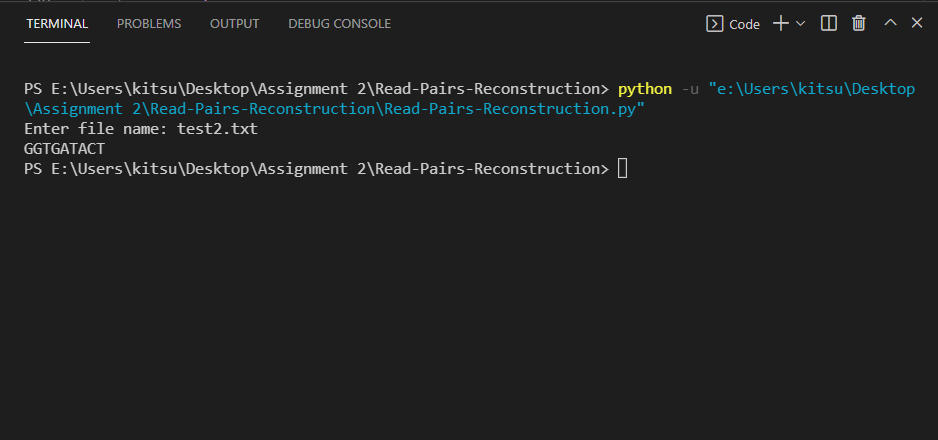
\includegraphics[scale=0.5]{ExampleInput2.png}\\
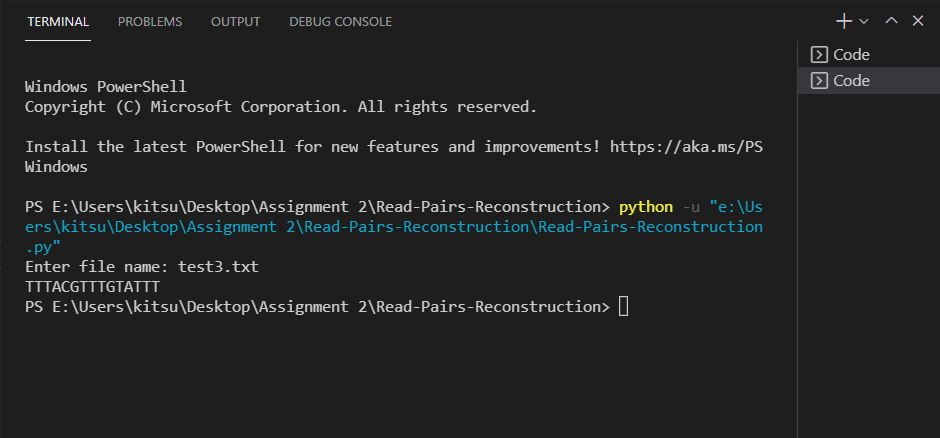
\includegraphics[scale=0.5]{ExampleInput3.png}\\

\end{document}
